% =====================================================================
%  Football Simulator : rapport d'état de l'art
%  Compilation : latexmk -pdf etat_de_l_art.tex   (pdfLaTeX)
% =====================================================================
\documentclass[11pt,a4paper]{article}

% ---------- Langue et polices ----------
\usepackage[utf8]{inputenc}
\usepackage[T1]{fontenc}
\usepackage{lmodern}
\usepackage[french]{babel}
\frenchsetup{SmallCapsFigTabCaptions=false}
\usepackage{microtype}
\usepackage{csquotes}

% ---------- Mise en page ----------
\usepackage[a4paper,margin=2.5cm,headheight=14pt]{geometry}
\usepackage{fancyhdr}
\usepackage{titlesec}
\usepackage{enumitem}
\usepackage{float}

% ---------- Couleurs, figures, tableaux ----------
\usepackage[table]{xcolor}
\usepackage{graphicx}
\usepackage{tikz}
\usetikzlibrary{arrows.meta,positioning,calc,decorations.pathreplacing,babel}
\usepackage{booktabs,tabularx,array,multirow}
\usepackage{caption}
\usepackage{pifont}
\usepackage[most]{tcolorbox}
\usepackage{xurl}
\usepackage{hyperref}

% Couleurs du cahier des charges
\definecolor{terrain}{HTML}{146E3C}
\definecolor{terrainclair}{HTML}{DCF0E1}
\definecolor{bleu}{HTML}{4C4CFF}
\definecolor{rouge}{HTML}{FF4040}
\definecolor{passe}{HTML}{E67814}
\definecolor{gris}{HTML}{66706B}

\hypersetup{
  colorlinks=true, linkcolor=black, citecolor=terrain, urlcolor=terrain,
  pdftitle={Football Simulator : état de l'art},
  pdfauthor={Iyed Rachdi, Bilel Khlif, Ghassen Dallekji},
  pdfsubject={État de l'art des tableaux tactiques de football en réalité augmentée},
}

% Titres verts numérotés, comme dans le cahier
\titleformat{\section}{\Large\bfseries\color{terrain}}{\thesection.}{0.6em}{}
\titleformat{\subsection}{\large\bfseries\color{terrain}}{\thesubsection}{0.6em}{}
\titlespacing*{\section}{0pt}{1.4em}{0.8em}
\titlespacing*{\subsection}{0pt}{1.1em}{0.5em}

% En-tête et pied de page
\pagestyle{fancy}
\fancyhf{}
\fancyhead[L]{\small Football Simulator}
\fancyhead[R]{\small État de l'art}
\fancyfoot[C]{\thepage}
\renewcommand{\headrulewidth}{0.4pt}

\captionsetup{font=small,labelfont={bf,color=terrain},labelsep=endash}
\setlist{itemsep=2pt,topsep=4pt}
\setlength{\parindent}{0pt}
\setlength{\parskip}{5pt}
\renewcommand{\arraystretch}{1.25}

% Encadré vert (style « Problématique » du cahier)
\newtcolorbox{encadre}[1][]{colback=terrainclair,colframe=terrain,boxrule=0.6pt,arc=2pt,
  left=6pt,right=6pt,top=4pt,bottom=4pt,#1}

% Marques des tableaux comparatifs
\newcommand{\oui}{\textcolor{terrain}{\ding{51}}}
\newcommand{\non}{\textcolor{gris}{\ding{55}}}
% Demi-disque « partiel », dessiné une seule fois puis réutilisé (sûr dans les légendes)
\newsavebox{\partielbox}
\AtBeginDocument{\sbox{\partielbox}{\tikz[baseline=-0.55ex]{\fill[gris] (0,0) -- (90:0.75ex) arc (90:270:0.75ex) -- cycle;
  \draw[gris,line width=0.4pt] (0,0) circle (0.75ex);}}}
\DeclareRobustCommand{\partiel}{\usebox{\partielbox}}
\newcommand{\code}[1]{\texttt{#1}}
\newcolumntype{C}[1]{>{\centering\arraybackslash}p{#1}}
\newcolumntype{L}[1]{>{\raggedright\arraybackslash}p{#1}}
\newcolumntype{Y}{>{\raggedright\arraybackslash}X}
\newcolumntype{G}{>{\columncolor{terrainclair}\raggedright\arraybackslash}X}

% =====================================================================
\begin{document}

% ---------- Page de garde ----------
\begin{titlepage}
  \centering
  {\large\bfseries SUP'COM\par}
  \vspace{2pt}
  {\normalsize Département SIA\par}
  \vspace{2.2cm}

  % Terrain vu de dessus : Bleus en 4-3-3, Rouges en 4-4-2 (positions du prototype)
  \begin{tikzpicture}[x=0.064cm,y=0.064cm]
    \fill[terrain] (-4,-4) rectangle (109,72);
    \begin{scope}[white,line width=0.8pt]
      \draw (0,0) rectangle (105,68);
      \draw (52.5,0) -- (52.5,68);
      \draw (52.5,34) circle (9.15);
      \draw (0,13.84) rectangle (16.5,54.16);
      \draw (105,13.84) rectangle (88.5,54.16);
      \draw (0,24.84) rectangle (5.5,43.16);
      \draw (105,24.84) rectangle (99.5,43.16);
    \end{scope}
    \fill[white] (52.5,34) circle (0.7);
    \foreach \x/\y in {4.2/34, 17.85/59.84, 17.85/42.84, 17.85/25.16, 17.85/8.16,
                       32.55/47.6, 28.35/34, 32.55/20.4, 45.15/58.48, 42/34, 45.15/9.52}
      \fill[bleu,draw=white,line width=0.4pt] (\x,\y) circle (1.9);
    \foreach \x/\y in {100.8/34, 87.15/8.16, 87.15/25.16, 87.15/42.84, 87.15/59.84,
                       72.45/8.16, 72.45/25.16, 72.45/42.84, 72.45/59.84, 57.75/25.84, 57.75/42.16}
      \fill[rouge,draw=white,line width=0.4pt] (\x,\y) circle (1.9);
    \draw[passe,line width=1.3pt,-{Latex[length=2.4mm]}] (30.2,36.9) -- (43.4,55.6);
  \end{tikzpicture}

  \vspace{1.6cm}
  {\fontsize{30}{36}\selectfont\bfseries\color{terrain} FOOTBALL SIMULATOR\par}
  \vspace{6pt}
  {\large Tableau tactique de football en Réalité Augmentée\par}
  \vspace{1.2cm}
  {\Large\bfseries État de l'art\par}
  \vspace{4pt}
  {\normalsize Solutions existantes, briques réutilisables et positionnement du projet\par}
  \vspace{2pt}
  {\normalsize Projet : WebXR AR \& Spatial Computing\par}
  \vfill
  \begin{minipage}[t]{0.48\textwidth}\raggedright
    \textbf{Équipe :}\\[2pt]
    Iyed Rachdi\\ Bilel Khlif\\ Ghassen Dallekji
  \end{minipage}\hfill
  \begin{minipage}[t]{0.48\textwidth}\raggedleft
    \textbf{Superviseur :}\\[2pt]
    Dr. Ing. Mohamed-Bécha Kaâniche
  \end{minipage}

  \vspace{1.4cm}
  {Année universitaire 2026 -- 2027\par}
  \vspace{2pt}
  {\small\color{gris} Version du 5 novembre 2026\par}
\end{titlepage}

% ---------- Sommaire ----------
\tableofcontents
\newpage

% =====================================================================
\section{Introduction}

Ce rapport fait l'état de l'art des solutions proches de Football Simulator, une application web de réalité augmentée qui pose un tableau tactique de football en 3D sur une vraie table. Il répond à trois questions : qu'existe-t-il déjà, que pouvons-nous réutiliser, et où se place notre projet ?

\begin{encadre}
\textbf{Synthèse :} aucune solution recensée ne réunit les trois propriétés visées par le projet, à savoir un terrain en AR posé sur une surface réelle, un accès par simple lien web et la gratuité. Le projet occupe donc un espace libre, mais il peut s'appuyer sur des briques existantes : l'exemple \code{webxr\_ar\_hittest} de three.js pour BF1 à BF3, les 13 formations de boardx pour BF4 et les données ouvertes de SkillCorner pour le bonus BF9.
\end{encadre}

\subsection{Rappel du besoin}

D'après le cahier des charges (§1.2), la plupart des entraîneurs amateurs expliquent encore la tactique sur un tableau blanc ou magnétique. Ce support n'offre qu'une vue de dessus en 2D, représente mal les déplacements, ne se partage pas à distance, et les logiciels d'analyse 3D restent coûteux et réservés aux clubs professionnels.

Football Simulator répond par une application web progressive (PWA) : un mini-terrain d'environ 60 × 40 cm s'affiche sur une table à travers la caméra d'un smartphone Android, depuis une URL ou un QR code. La figure~\ref{fig:prototype} montre le prototype livré au sprint 1, dans sa vue 3D hors AR.

\begin{figure}[H]
  \centering
  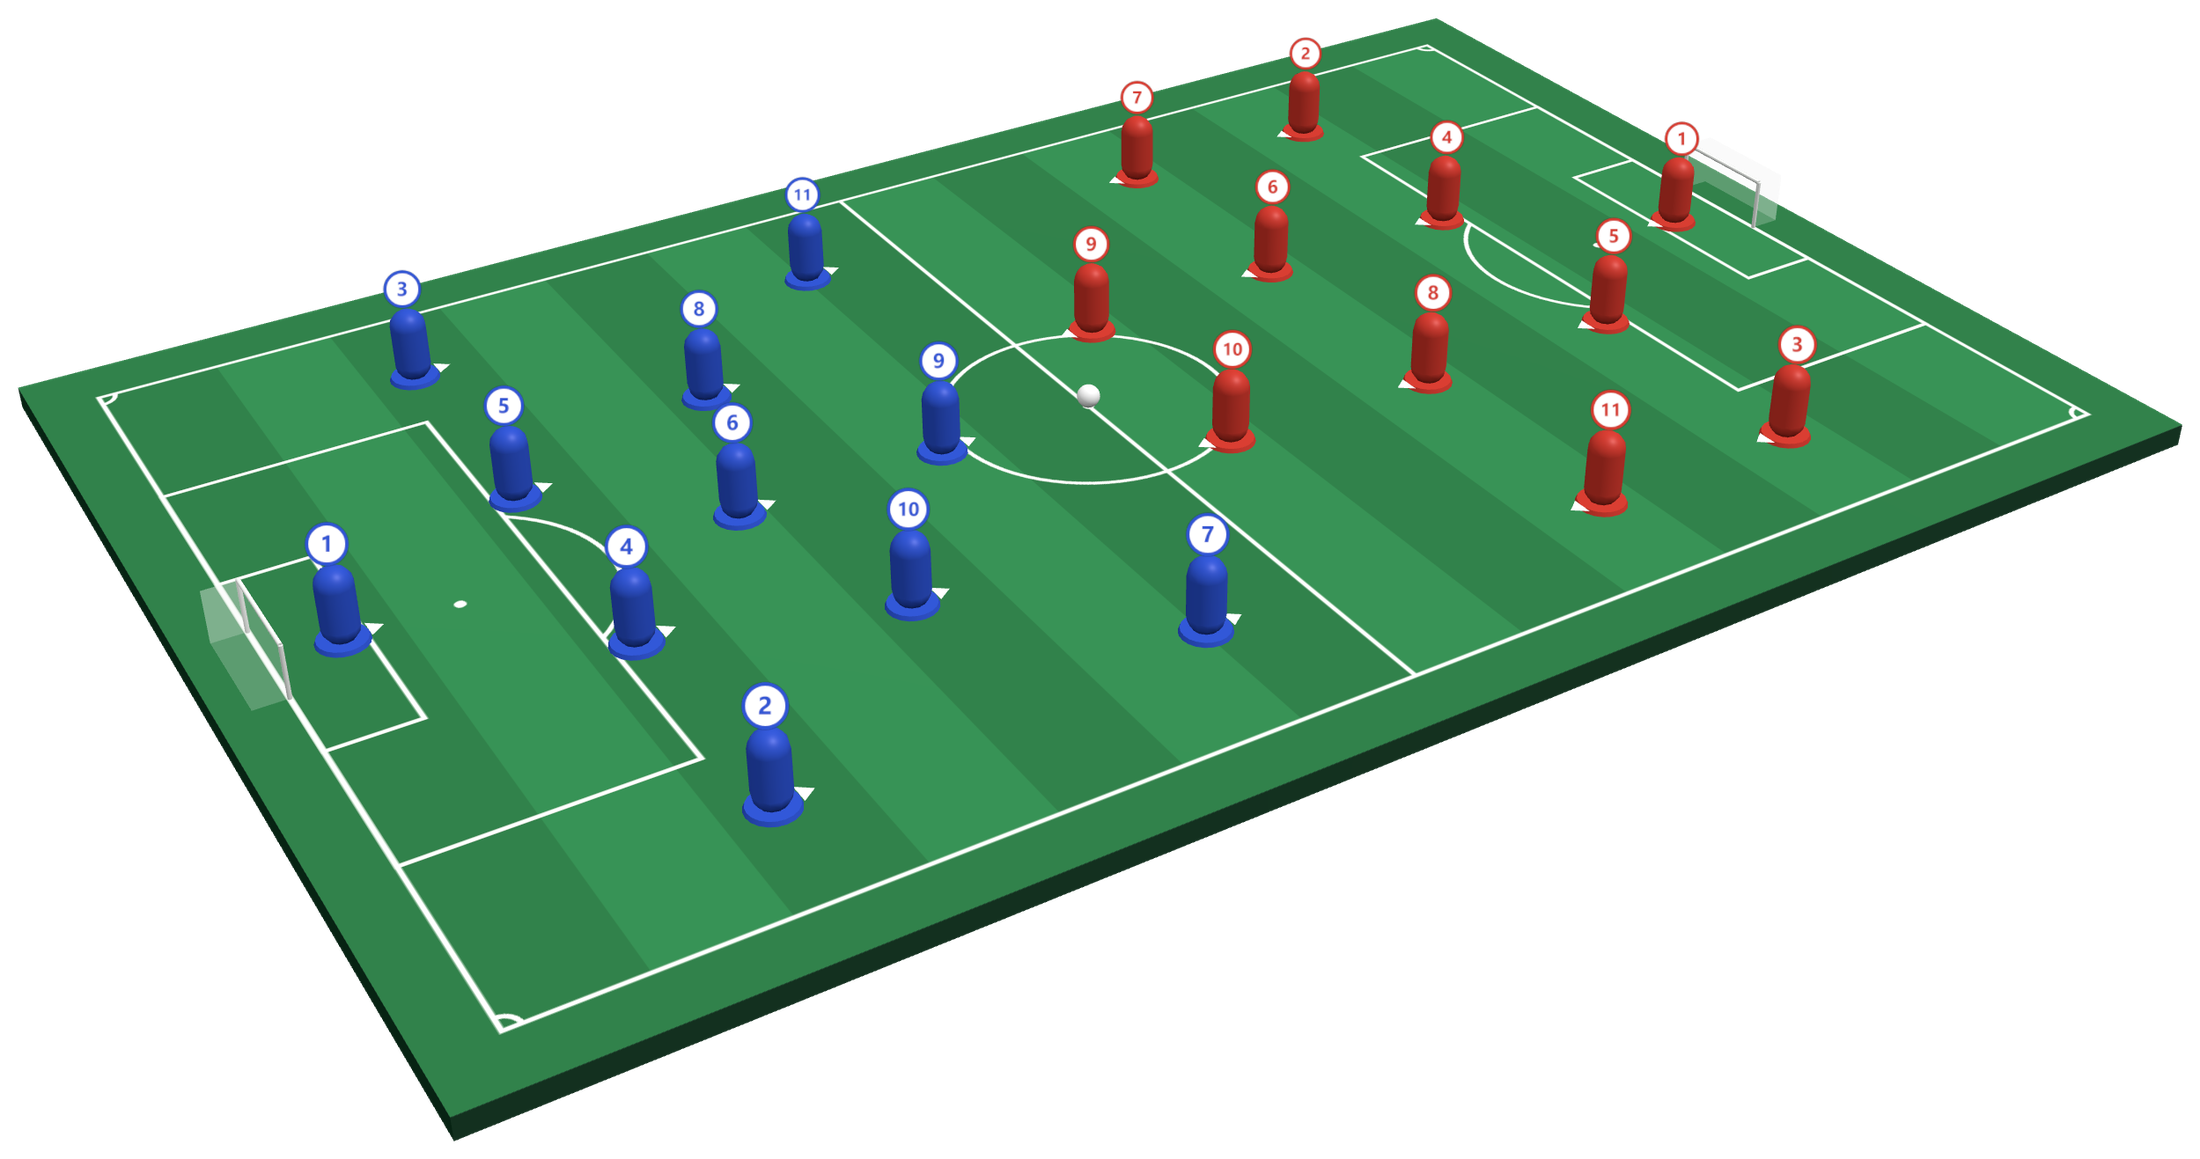
\includegraphics[width=0.72\textwidth]{figures/prototype-3d.png}\hfill
  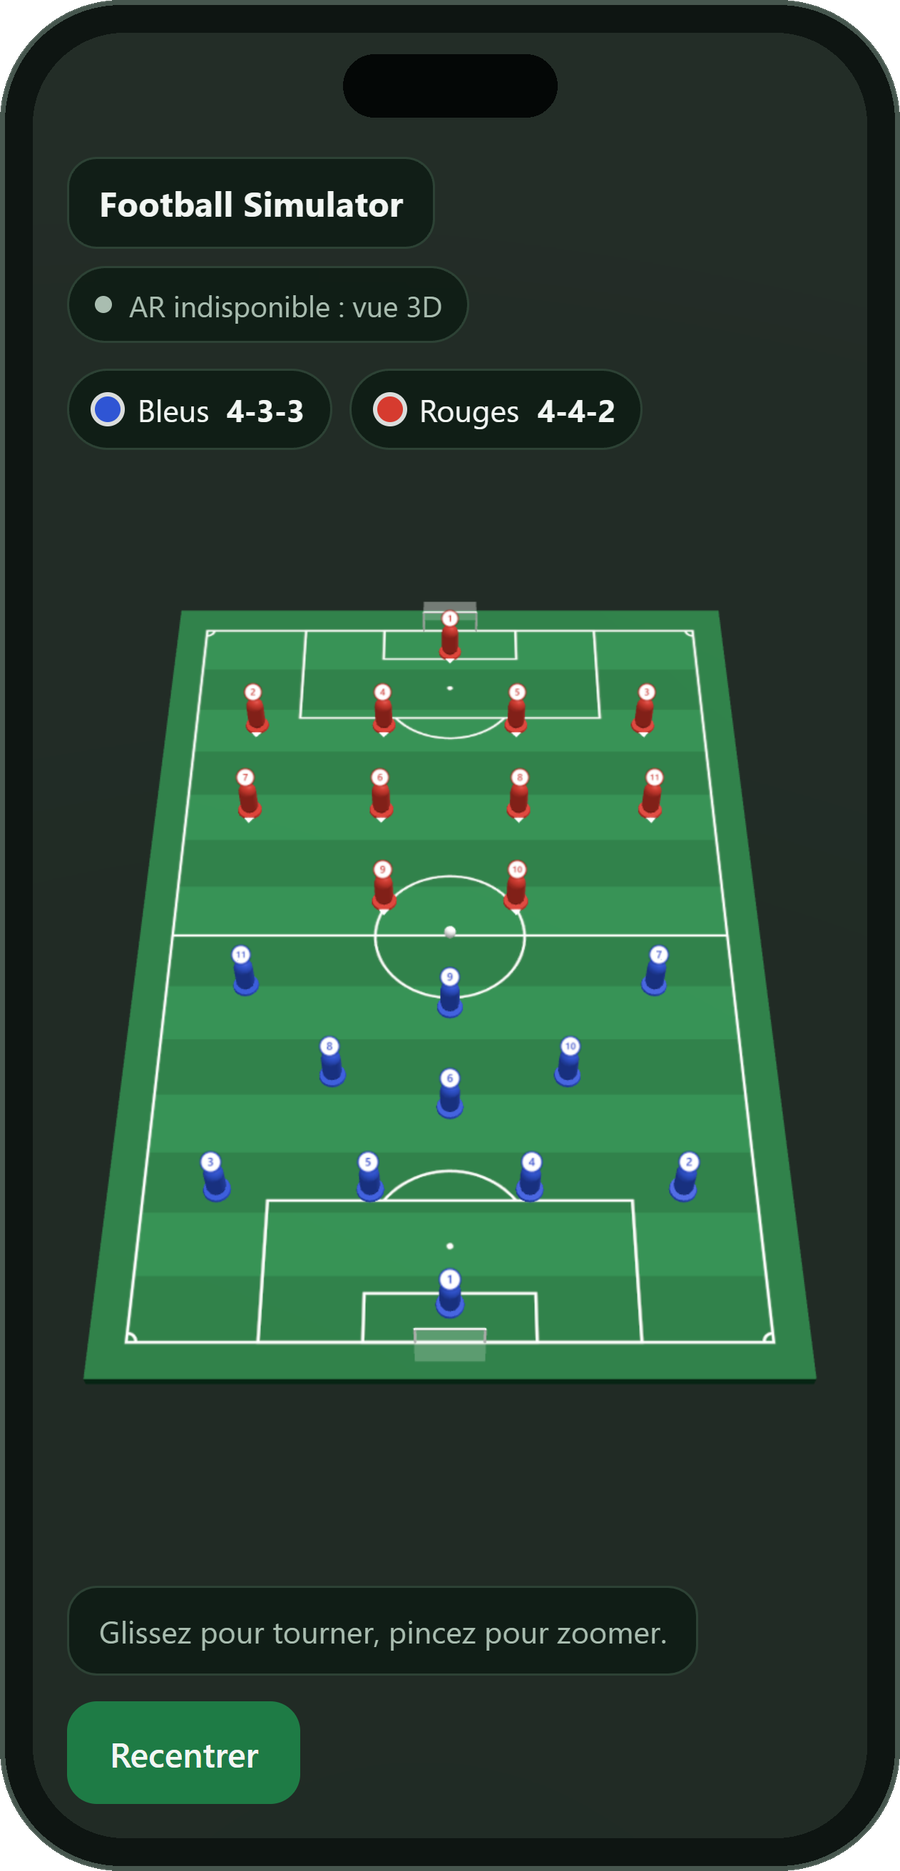
\includegraphics[height=6.2cm]{figures/prototype-mobile.png}
  \caption{Prototype du sprint 1 : terrain de 60 × 39 cm, Bleus en 4-3-3 et Rouges en 4-4-2 (à gauche), et interface sur mobile (à droite).}
  \label{fig:prototype}
\end{figure}

\subsection{Démarche et critères}

La veille couvre quatre familles de solutions : les tableaux tactiques numériques, les travaux de recherche sur l'AR appliquée à la tactique, les briques techniques WebXR, et la vision par ordinateur avec les jeux de données de suivi des joueurs. Les sources (dépôts GitHub, articles arXiv, pages produits et dépôts de données) ont été consultées le 5 novembre 2026. Chaque solution est jugée selon les sept critères du tableau~\ref{tab:criteres}, tous tirés du cahier.

\begin{table}[H]
  \centering
  \caption{Critères d'évaluation tirés du cahier des charges.}
  \label{tab:criteres}
  \begin{tabularx}{\textwidth}{L{4.2cm}YC{2.2cm}}
    \toprule
    \textbf{Critère} & \textbf{Exigence} & \textbf{Référence} \\
    \midrule
    AR sur une surface réelle & Session \code{immersive-ar}, hit test et ancrage du terrain & BF1--BF3, §1.4 \\
    Accès sans installation & Simple URL ou QR code, application PWA & §2.3 \\
    Gratuité & Outils libres ou gratuits, budget nul & §1.1 \\
    Formations & 4-4-2, 4-3-3 et 3-5-2 pour chaque équipe & BF4 \\
    Manipulation & Déplacer joueurs et ballon, tracer des flèches, annuler & BF5--BF8 \\
    Animation & Rejouer une action pas à pas & BF9 (bonus) \\
    Hors-ligne & Fonctionnement après le premier chargement & §2.3 \\
    \bottomrule
  \end{tabularx}
\end{table}

% =====================================================================
\section{Tableaux tactiques numériques}

Aucun des sept tableaux recensés ne pose un terrain en AR sur une surface réelle. Les trois projets dont le code est public sont en 2D, et la 3D n'apparaît que dans des produits commerciaux (tableau~\ref{tab:tableaux}).

\begin{table}[H]
  \centering
  \caption{Tableaux tactiques numériques recensés.}
  \label{tab:tableaux}
  \small
  \begin{tabularx}{\textwidth}{L{3.6cm}YC{1.9cm}L{3.3cm}}
    \toprule
    \textbf{Solution} & \textbf{Plateforme} & \textbf{Rendu} & \textbf{Licence ou prix} \\
    \midrule
    \multicolumn{4}{l}{\footnotesize\bfseries\color{terrain} CODE PUBLIC} \\
    boardx~\cite{boardx} & Web : React 19, Konva, Zustand & 2D & MIT \\
    soccer-tactics-board~\cite{stboard} & Web : TypeScript et Canvas 2D & 2D & Aucune licence affichée \\
    Sports Tactics Board~\cite{sportstb} & Windows, .NET 3.5 & 2D & GPL v2 \\
    \midrule
    \multicolumn{4}{l}{\footnotesize\bfseries\color{terrain} COMMERCIAL} \\
    TacticSlate~\cite{tacticslate} & Web & 2D et 3D & Prix non publié \\
    FC Tactix~\cite{fctactix} & Plateforme de coaching & 2D et 3D & Prix non publié \\
    SoccerBoard Tactics AI~\cite{soccerboard} & iPhone & Effet 3D & Achat unique \\
    TacticalPad~\cite{tacticalpad} & macOS & 2D et 3D & 39,99 USD par an \\
    \bottomrule
  \end{tabularx}
\end{table}

\textbf{Projets au code public.} boardx propose 13 formations prédéfinies (dont le 4-3-3, le 4-4-2 et le 3-5-2), une animation par images clés avec une interpolation \code{easeInOutQuad} et des exports PNG, WebM et GIF. soccer-tactics-board enregistre les positions étape par étape en JSON et les interpole pour l'animation, mais le dépôt n'affiche aucune licence. Sports Tactics Board est un logiciel Windows au style de tableau magnétique, qui enregistre des séquences de positions.

\textbf{Produits commerciaux.} TacticSlate fonctionne dans le navigateur avec des vues 2D et 3D et des positions \enquote{fantômes} entre les images clés. FC Tactix ajoute la génération d'actions par IA à partir d'un texte. SoccerBoard Tactics AI donne aux pions un effet de volume sur iPhone, et TacticalPad propose une 3D réaliste sur macOS par abonnement.

\textbf{Ce que nous retenons.} Les coordonnées des 13 formations de boardx, sous licence MIT, peuvent nourrir les stratégies de \code{formations.js} (BF4). Le format d'étapes de soccer-tactics-board inspire le bouton \enquote{Play} (BF9), comme idée seulement, faute de licence.

% =====================================================================
\section{Réalité augmentée et tactique sportive dans la recherche}

La recherche confirme l'intérêt de l'AR mobile pour expliquer une tactique, mais aucun des quatre travaux recensés ne propose un tableau manipulable dans le navigateur. Ils reposent sur un casque, une application native ou un concept non publié (tableau~\ref{tab:recherche}).

\begin{table}[H]
  \centering
  \caption{Travaux de recherche et projets académiques.}
  \label{tab:recherche}
  \small
  \begin{tabularx}{\textwidth}{L{3.3cm}C{1.3cm}YL{2.6cm}}
    \toprule
    \textbf{Travail} & \textbf{Année} & \textbf{Dispositif et apport} & \textbf{Code} \\
    \midrule
    Collaborative XRTactics~\cite{xrtactics} & 2024 & Étude formative : plateforme web pour l'entraîneur, application AR mobile pour les joueurs, encore en développement & Non publié \\
    PanoCoach~\cite{panocoach} & 2024 & Unity, WebXR et Photon PUN2, testé sur Oculus Quest 2 ; l'entraîneur annote sur une tablette 2D, les joueurs voient la tactique en vue subjective & Non publié \\
    Soccer On Your Tabletop~\cite{tabletop} & 2018 & Match YouTube converti en scène 3D (Mask R-CNN, OpenPose, calibration, profondeur), regardé sur HoloLens & BSD-2, non maintenu \\
    TactiQuest~\cite{tactiquest} & 2024--25 & Application AR qui reconnaît un terrain imprimé ; défis tactiques par niveaux pour les 12--16 ans & Pas de sortie publique \\
    \bottomrule
  \end{tabularx}
\end{table}

\begin{encadre}
\textbf{Résultat clé :} dans l'enquête de Collaborative XRTactics, 12 joueurs de Division I sur 17 préfèrent l'AR mobile au tableau tactique classique, et 5 préfèrent le tableau. Les casques de réalité mixte ou virtuelle sont écartés pour des raisons de confort et de praticité~\cite{xrtactics}.
\end{encadre}

PanoCoach a recueilli les retours qualitatifs d'entraîneurs et d'analystes de City Football Group, de Harvard Soccer et de Rice Soccer, sans mesure chiffrée ; ses joueurs virtuels sont encore déplacés à la main~\cite{panocoach}. Soccer On Your Tabletop reste la référence historique du \enquote{match sur la table}, mais son pipeline lourd et son code non maintenu le rendent difficile à réutiliser~\cite{tabletop}. Ces résultats justifient directement la problématique du cahier : un smartphone suffit, et il est préféré au casque.

% =====================================================================
\section{Briques techniques WebXR}

\subsection{Bibliothèques et approches}

three.js reste le meilleur socle pour le cahier : il fournit un exemple complet de hit test et laisse chaque API WebXR visible. Les alternatives masquent ces API, limitent l'interaction en AR ou imposent une installation (tableau~\ref{tab:bibliotheques}).

\begin{table}[H]
  \centering
  \caption{Comparaison des approches techniques (\oui~oui, \partiel~partiel, \non~non).}
  \label{tab:bibliotheques}
  \small
  \setlength{\tabcolsep}{4pt}
  \begin{tabular}{L{3.4cm}C{1.45cm}C{1.45cm}C{1.45cm}C{1.2cm}C{1.45cm}C{1.45cm}C{1.35cm}}
    \toprule
    \textbf{Approche} & \footnotesize\textbf{Pose sur surface} & \footnotesize\textbf{Inter\-action libre} & \footnotesize\textbf{Sans instal\-lation} & \footnotesize\textbf{Gratuit} & \footnotesize\textbf{Toujours actif} & \footnotesize\textbf{Imposé par le cahier} & \textbf{Verdict} \\
    \midrule
    \rowcolor{terrainclair} three.js + WebXR~\cite{threejs} & \oui & \oui & \oui & \oui & \oui & \oui & \textbf{\color{terrain}Retenu} \\
    A-Frame 1.8.0~\cite{aframe} & \oui & \oui & \oui & \oui & \oui & \non & Possible \\
    Babylon.js~\cite{babylon} & \oui & \oui & \oui & \oui & \oui & \non & Possible \\
    model-viewer~\cite{modelviewer} & \oui & \partiel & \oui & \oui & \oui & \non & Écarté \\
    8th Wall~\cite{eighthwall} & \oui & \oui & \oui & \partiel & \non & \non & Écarté \\
    SDK natifs (ARCore, Unity) & \oui & \oui & \non & \oui & \oui & \non & Écarté \\
    \bottomrule
  \end{tabular}
\end{table}

A-Frame (licence MIT) est une couche fine au-dessus de three.js, avec un composant \code{ar-hit-test} prêt à l'emploi, mais la session et le hit test disparaissent derrière des balises HTML. Babylon.js (Apache 2.0) est un moteur complet, plus lourd et hors du programme du cours. model-viewer (Google, Apache 2.0) affiche un modèle en AR via WebXR sur Chrome Android, Scene Viewer ou Quick Look sur iOS, mais il ne prévoit pas la sélection de 22 joueurs. Enfin, Niantic Spatial a fermé les services hébergés de 8th Wall en 2026 et publié son moteur sous licence MIT, mais le SLAM n'existe qu'en binaire~\cite{eighthwall}. Les SDK natifs exigent une installation, contraire au §2.3 du cahier.

\subsection{Compatibilité des navigateurs}

Selon Can I use~\cite{caniuse}, WebXR n'est que partiellement pris en charge, et uniquement par les navigateurs Chromium sur Android (tableau~\ref{tab:navigateurs}). Le choix de Chrome Android avec ARCore, fait au cahier (§6.1), est donc le bon. L'API a toutefois atteint le stade de recommandation candidate du W3C et figure parmi les priorités d'Interop 2026~\cite{vrorg}.

\begin{table}[H]
  \centering
  \caption{Prise en charge de l'API WebXR, novembre 2026.}
  \label{tab:navigateurs}
  \small
  \begin{tabularx}{0.82\textwidth}{L{4cm}YC{1.2cm}}
    \toprule
    \textbf{Navigateur} & \textbf{Prise en charge} & \\
    \midrule
    Chrome Android & Partielle, sur un appareil compatible ARCore & \oui \\
    Samsung Internet & Partielle, versions 12 à 31 & \oui \\
    Safari sur iOS & Non prise en charge, jusqu'à la version 27.2 & \non \\
    Firefox & Désactivée par défaut & \non \\
    \bottomrule
  \end{tabularx}
\end{table}

\subsection{Exemples réutilisables}

\begin{itemize}
  \item \textbf{\code{webxr\_ar\_hittest} (three.js)}~\cite{threehittest} : bouton AR exigeant la fonctionnalité \code{hit-test}, réticule en anneau et pose d'un objet au tap. Il couvre BF1 à BF3 ; l'objet posé devient notre groupe \code{pitchGroup}.
  \item \textbf{\code{hit-test-anchors} (W3C Immersive Web)}~\cite{webxrsamples} : création d'un \code{XRAnchor} depuis un résultat de hit test, puis mise à jour de sa pose à chaque image. Son nettoyage de fin de session appelle \code{clear()} sur un tableau JavaScript, ce qui échoue : cette partie ne doit pas être copiée.
  \item \textbf{Tutoriel \enquote{Hello WebXR} d'ARCore}~\cite{arcore} : la même chaîne pas à pas avec three.js, sans ancres.
\end{itemize}

\subsection{Outils de test sans téléphone}

L'Immersive Web Emulator, solution de secours prévue au §4.2 du cahier, est archivé depuis le 1\ier{} octobre 2026 et n'émulait pas le DOM Overlay~\cite{iwe}. Nous l'avons remplacé au sprint 1 par son moteur, IWER~\cite{iwer}, dans sa version 2.7.0 ; la version 2.8.0, publiée la veille, n'a pas été retenue. Le tableau~\ref{tab:iwer} résume ce que nous avons vérifié avec Chrome 156 sur PC.

\begin{table}[H]
  \centering
  \caption{Capacités d'IWER vérifiées au sprint 1.}
  \label{tab:iwer}
  \small
  \begin{tabularx}{0.82\textwidth}{YC{1.2cm}}
    \toprule
    \textbf{Fonction émulée} & \\
    \midrule
    Ouverture d'une session \code{immersive-ar}, en mode \code{alpha-blend} & \oui \\
    Espace de référence \code{local-floor} et ancres & \oui \\
    Hit test : refusé sans le module d'environnement synthétique \code{@iwer/sem} & \non \\
    DOM Overlay & \non \\
    \bottomrule
  \end{tabularx}
\end{table}

Chrome sur PC expose déjà un \code{navigator.xr} natif sans AR : IWER doit donc être installé en mode forcé, ce que notre code ne fait qu'après avoir vérifié que l'AR native est absente.

% =====================================================================
\section{Vision par ordinateur et données de suivi}

\subsection{Le pipeline vidéo}

Le post LinkedIn de Shabahang Shayegan qui a inspiré l'équipe montre une attaque de Chelsea à l'Emirates : joueurs détectés et nommés, ballon suivi et carte 2D des positions, à partir de la seule vidéo TV~\cite{linkedin}. Aucun code n'est publié, et des commentateurs signalent des échanges d'identité quand les joueurs se masquent. Football-PitchVision, dérivé de roboflow/sports, détaille le pipeline nécessaire (figure~\ref{fig:pipeline})~\cite{pitchvision,roboflow}.

\begin{figure}[H]
  \centering
  \begin{tikzpicture}[node distance=2.8mm,
      etape/.style={draw=gris!60,rounded corners=2pt,minimum width=2.33cm,minimum height=1.25cm,align=center,font=\small},
      fleche/.style={-{Latex[length=1.8mm]},gris}]
    \node[etape] (a) {\textbf{Vidéo TV}\\[-1pt]{\footnotesize match diffusé}};
    \node[etape,right=of a] (b) {\textbf{Détection}\\[-1pt]{\footnotesize YOLOv8}};
    \node[etape,right=of b] (c) {\textbf{Suivi}\\[-1pt]{\footnotesize ByteTrack}};
    \node[etape,right=of c] (d) {\textbf{Équipes}\\[-1pt]{\footnotesize SigLIP, UMAP,}\\[-3pt]{\footnotesize KMeans}};
    \node[etape,right=of d] (e) {\textbf{Calibration}\\[-1pt]{\footnotesize homographie}};
    \node[etape,right=of e,fill=terrainclair,draw=terrain] (f) {\textbf{\color{terrain}Carte 2D}\\[-1pt]{\footnotesize vue radar}};
    \foreach \u/\v in {a/b,b/c,c/d,d/e,e/f} \draw[fleche] (\u) -- (\v);
    \draw[decorate,decoration={brace,mirror,amplitude=5pt},gris]
      ([yshift=-2.5mm]a.south west) -- ([yshift=-2.5mm]e.south east)
      node[midway,below=6pt,font=\footnotesize,text=gris] {Hors périmètre : un projet de vision par ordinateur à part entière};
    \node[below=7mm of f,font=\footnotesize\bfseries,text=terrain,align=center] {Seule sortie\\utile au tableau};
  \end{tikzpicture}
  \caption{Pipeline d'analyse vidéo de Football-PitchVision.}
  \label{fig:pipeline}
\end{figure}

Ce pipeline sort du périmètre du cahier, qui exclut l'intelligence artificielle (§2.5), et du module, qui porte sur WebXR. Football-PitchVision ne produit d'ailleurs qu'une vidéo annotée : l'export JSON ou CSV figure dans sa feuille de route sans être implémenté, et les poids YOLOv8 sont sous licence AGPL-3.0~\cite{pitchvision}. Seule la sortie du pipeline, la position des joueurs, intéresse notre tableau.

\subsection{Jeux de données ouverts}

Ces positions existent déjà en données ouvertes. SkillCorner est la seule source qui combine un suivi tiré de la vidéo TV, des coordonnées en mètres et une licence MIT (tableau~\ref{tab:donnees}).

\begin{table}[H]
  \centering
  \caption{Jeux de données de suivi des joueurs.}
  \label{tab:donnees}
  \small
  \begin{tabularx}{\textwidth}{L{2.3cm}GYY}
    \toprule
    & \textbf{\color{terrain}SkillCorner~\cite{skillcorner}} & \textbf{Metrica Sports~\cite{metrica}} & \textbf{StatsBomb~\cite{statsbomb}} \\
    \midrule
    \textbf{Contenu} & 10 matchs d'A-League 2024/25 & 3 matchs, avec leurs événements & Événements, compositions, données 360 \\
    \textbf{Suivi} & Tiré de la vidéo TV, 10 images par seconde & Synchronisé avec les événements & Lié aux événements, pas image par image \\
    \textbf{Coordonnées} & En mètres, origine au centre du terrain & De 0 à 1, terrain de 105 × 68 m & Non précisé sur le dépôt \\
    \textbf{Conditions} & MIT, citer SkillCorner & Pas de licence nommée, citer la source & \code{LICENSE.pdf}, citer avec le logo \\
    \bottomrule
  \end{tabularx}
\end{table}

\subsection{Utilisation proposée}

Le rejeu d'une action réelle peut devenir une variante bonus de BF9, sans aucune intelligence artificielle :
\begin{enumerate}
  \item un script hors ligne extrait une action d'environ 15 secondes d'un match SkillCorner (fichier JSONL) ;
  \item il la convertit au format d'étapes du bouton \enquote{Play} ;
  \item une échelle de 0,6/105 ramène le terrain réel à 60 × 39 cm ;
  \item le fichier rejoint le dossier \code{/assets} et reste disponible hors-ligne.
\end{enumerate}
Les joueurs estimés hors champ (\code{is\_detected} à faux) peuvent être affichés en transparence. SkillCorner annonce environ 97\,\% d'identités correctes : l'extrait devra être vérifié à l'œil~\cite{skillcorner}.

% =====================================================================
\section{Analyse comparative}

Parmi les dix solutions placées sur la figure~\ref{fig:positionnement}, aucune ne combine la réalité augmentée et l'accès par lien web : seul Football Simulator occupe cette zone. Les positions indiquent une zone, pas un score ; FC Tactix n'est pas placé, car sa plateforme n'est pas précisée.

\begin{figure}[H]
  \centering
  \begin{tikzpicture}[x=1cm,y=1cm,font=\small]
    % Zone visée par le projet, puis les deux axes (croisement en (7.75, 3.6))
    \fill[terrainclair] (7.85,3.7) rectangle (15.6,7.2);
    \draw[gris,-{Latex[length=2mm]}] (0,3.6) -- (15.7,3.6);
    \draw[gris,-{Latex[length=2mm]}] (7.75,0) -- (7.75,7.3);
    \node[anchor=south west,font=\footnotesize,text=gris] at (0,3.62) {Application ou matériel à installer};
    \node[anchor=north east,font=\footnotesize,text=gris] at (15.7,3.55) {Lien web sur smartphone};
    \node[anchor=south east,font=\footnotesize,text=gris] at (7.65,6.95) {Immersif : AR ou casque};
    \node[anchor=south east,font=\footnotesize,text=gris] at (7.65,0) {Sur écran, en 2D ou 3D};
    % Haut gauche
    \node[anchor=west,font=\footnotesize\bfseries,text=gris] at (0.2,6.75) {IMMERSIF, À INSTALLER};
    \node[anchor=west] at (0.2,6.2) {\textbullet~Soccer On Your Tabletop~~{\footnotesize\color{gris}HoloLens, 2018}};
    \node[anchor=west] at (0.2,5.7) {\textbullet~PanoCoach~~{\footnotesize\color{gris}casque Quest 2, 2024}};
    \node[anchor=west] at (0.2,5.2) {\textbullet~XRTactics~~{\footnotesize\color{gris}application AR mobile, 2024}};
    \node[anchor=west] at (0.2,4.7) {\textbullet~TactiQuest~~{\footnotesize\color{gris}application AR, 2024--25}};
    % Bas gauche
    \node[anchor=west,font=\footnotesize\bfseries,text=gris] at (0.2,2.95) {SUR ÉCRAN, À INSTALLER};
    \node[anchor=west] at (0.2,2.4) {\textbullet~TacticalPad~~{\footnotesize\color{gris}macOS, 2D et 3D}};
    \node[anchor=west] at (0.2,1.9) {\textbullet~SoccerBoard Tactics AI~~{\footnotesize\color{gris}iPhone, effet 3D}};
    \node[anchor=west] at (0.2,1.4) {\textbullet~Sports Tactics Board~~{\footnotesize\color{gris}Windows, 2D}};
    % Bas droite
    \node[anchor=west,font=\footnotesize\bfseries,text=gris] at (8.1,2.95) {SUR ÉCRAN, DANS LE NAVIGATEUR};
    \node[anchor=west] at (8.1,2.4) {\textbullet~boardx~~{\footnotesize\color{gris}2D, MIT}};
    \node[anchor=west] at (8.1,1.9) {\textbullet~soccer-tactics-board~~{\footnotesize\color{gris}2D, sans licence}};
    \node[anchor=west] at (8.1,1.4) {\textbullet~TacticSlate~~{\footnotesize\color{gris}2D et 3D}};
    % Haut droite : le projet
    \node[anchor=west,font=\footnotesize\bfseries,text=terrain] at (8.1,6.75) {IMMERSIF, PAR LIEN WEB};
    \fill[terrain,opacity=0.18] (8.55,6.05) circle (0.3);
    \fill[terrain] (8.55,6.05) circle (0.12);
    \node[anchor=west,font=\large\bfseries,text=terrain] at (8.95,6.07) {Football Simulator};
    \node[anchor=north west,align=left,text width=6.3cm] at (8.95,5.7) {WebXR et three.js sur Chrome Android, PWA ouverte par une URL ou un QR code};
    \node[anchor=west,font=\footnotesize\itshape,text=gris] at (8.95,4.05) {Aucune autre solution recensée ici};
  \end{tikzpicture}
  \caption{Positionnement des solutions recensées selon l'accès et le mode d'affichage.}
  \label{fig:positionnement}
\end{figure}

% =====================================================================
\section{Ce que nous réutilisons}

Six briques existantes couvrent une partie des besoins BF1 à BF9 (tableau~\ref{tab:reutilisation}). Toutes sont sous licence MIT, ou ne sont reprises que comme idées, ce qui respecte le budget nul.

\begin{table}[H]
  \centering
  \caption{Briques réutilisées, besoins couverts et sprint d'intégration.}
  \label{tab:reutilisation}
  \small
  \begin{tabularx}{\textwidth}{L{3.6cm}L{2.6cm}C{1.9cm}C{1.3cm}Y}
    \toprule
    \textbf{Brique} & \textbf{Source et licence} & \textbf{Besoin} & \textbf{Sprint} & \textbf{Mode de réutilisation} \\
    \midrule
    IWER 2.7.0 & Meta, MIT & Tests sur PC (§4.2) & S1 & Dépendance de développement, activée par \code{?iwer} \\
    Exemple \code{webxr\_ar\_hittest} & three.js, MIT & BF1--BF3 & S2--S3 & Code adapté : l'objet posé devient \code{pitchGroup} \\
    Échantillon \code{hit-test-anchors} & Immersive Web, MIT & Ancrage (§3.3) & S3 & Logique reprise, nettoyage corrigé \\
    13 formations & boardx, MIT & BF4 & S4 & Coordonnées converties en stratégies \\
    Étapes et \code{easeInOutQuad} & soccer-tactics-board, boardx & BF9 & S6 & Principe réécrit, aucun code copié sans licence \\
    Extrait de match & SkillCorner, MIT & BF9 (bonus) & S6 & Données converties par un script hors ligne \\
    \bottomrule
  \end{tabularx}
\end{table}

Restent à développer par l'équipe : la sélection par raycasting (BF5 et BF6), les flèches (BF7) et l'annulation (BF8). Le modèle 3D du terrain et des joueurs, les formations et le Service Worker ont été livrés au sprint 1.

% =====================================================================
\section{Risques et ajustements du cahier}

La veille révèle un risque que le cahier ne couvrait pas : sa solution de test sans téléphone est archivée. Cinq ajustements sont proposés à l'encadrant (tableau~\ref{tab:ajustements}) ; les deux premiers sont déjà appliqués dans le code du sprint 1.

\begin{table}[H]
  \centering
  \caption{Constats de la veille et ajustements proposés.}
  \label{tab:ajustements}
  \small
  \begin{tabularx}{\textwidth}{C{0.5cm}L{6.2cm}Y}
    \toprule
    & \textbf{Constat} & \textbf{Ajustement proposé} \\
    \midrule
    1 & L'Immersive Web Emulator est archivé et n'émule pas le DOM Overlay & Citer IWER aux §4.2 et §6.3 ; tester l'interface dans la vue 3D hors AR \\
    2 & Safari sur iOS ne prend pas en charge WebXR & Ouvrir la vue 3D quand \code{immersive-ar} manque ; prévoir un téléphone Android pour la démonstration \\
    3 & 8th Wall a fermé ses services, sans SLAM dans le code ouvert & Noter l'exclusion d'iOS dans les hypothèses (§6.2) \\
    4 & Le rejeu SkillCorner n'est pas prévu au cahier & L'ajouter comme variante bonus de BF9, avec l'accord de l'encadrant \\
    5 & soccer-tactics-board est publié sans licence & Réécrire le principe et citer la source dans la documentation \\
    \bottomrule
  \end{tabularx}
\end{table}

% =====================================================================
\section*{Conclusion}
\addcontentsline{toc}{section}{Conclusion}

Football Simulator comble un manque réel : un tableau tactique en réalité augmentée, gratuit et ouvert depuis un simple lien, n'existe ni en open source ni dans le commerce. La recherche confirme l'intérêt de l'AR sur smartphone, et les briques three.js, WebXR et boardx réduisent le risque technique sur BF1 à BF4.

Le rejeu d'actions réelles issues de SkillCorner offre une suite naturelle au projet. Il rapproche le tableau tactique de l'analyse vidéo, sans sortir du périmètre WebXR du module. Les prochaines étapes sont la validation des cinq ajustements du cahier, la session \code{immersive-ar} du sprint 2, testée avec IWER, puis le choix, au sprint 3, entre l'intégration de \code{@iwer/sem} et un test du hit test sur téléphone uniquement.

\vspace{0.6cm}
\begin{center}
  {\large\bfseries\color{terrain} Le terrain tient sur votre table : à vous de jouer la tactique !}
\end{center}

% =====================================================================
\newpage
\begin{thebibliography}{99}
\small
\setlength{\itemsep}{2pt}

\bibitem{boardx} caztangpro, \emph{boardx}, dépôt GitHub. \url{https://github.com/caztangpro/boardx}
\bibitem{stboard} kenzo0107, \emph{soccer-tactics-board}, dépôt GitHub et article de présentation, juin 2026. \url{https://github.com/kenzo0107/soccer-tactics-board}
\bibitem{sportstb} \emph{Sports Tactics Board}, SourceForge. \url{https://sportstacticsbd.sourceforge.net/}
\bibitem{tacticslate} \emph{TacticSlate}, fiche Product Hunt. \url{https://hunted.space/product/tacticslate}
\bibitem{fctactix} \emph{FC Tactix}, fiche Product Hunt, avril 2026. \url{https://hunted.space/product/fc-tactix}
\bibitem{soccerboard} \emph{SoccerBoard Tactics AI}, fiche d'application, avril 2026. \url{https://mwm.ai/apps/soccerboard-tactics-ai/6762029244}
\bibitem{tacticalpad} Temma Software, \emph{TacticalPad}, Mac App Store. \url{https://apps.apple.com/uz/app/tacticalpad/id946927077?mt=12}

\bibitem{xrtactics} U. Gong, Q. Zhang, Z. Yin, S. Zollmann, \emph{Collaborative XRTactics: A Formative Study on Tactical Communication in Outdoor Team Sports}, arXiv:2408.14305, 2024. \url{https://arxiv.org/html/2408.14305v1}
\bibitem{panocoach} A. Kang, H. Pfister, T. Lin, \emph{PanoCoach: Enhancing Tactical Coaching and Communication in Soccer with Mixed-Reality Telepresence}, arXiv:2409.13859, 2024. \url{https://arxiv.org/html/2409.13859v1}
\bibitem{tabletop} K. Rematas, I. Kemelmacher-Shlizerman, B. Curless, S. Seitz, \emph{Soccer On Your Tabletop}, CVPR 2018, code. \url{https://github.com/krematas/soccerontable}
\bibitem{tactiquest} S. Islam, \emph{TactiQuest}, Copenhagen Institute of Interaction Design, 2024--25. \url{https://www.ciid.dk/idp-projects/tactiquest}

\bibitem{threejs} \emph{three.js}, dépôt GitHub, licence MIT. \url{https://github.com/mrdoob/three.js}
\bibitem{threehittest} three.js, exemple \emph{webxr\_ar\_hittest}. \url{https://raw.githubusercontent.com/mrdoob/three.js/dev/examples/webxr_ar_hittest.html}
\bibitem{webxrsamples} Immersive Web Community Group, \emph{webxr-samples}, échantillon \emph{hit-test-anchors}. \url{https://github.com/immersive-web/webxr-samples}
\bibitem{aframe} \emph{A-Frame}, dépôt GitHub et composant \emph{ar-hit-test}. \url{https://aframe.io/docs/1.7.0/components/ar-hit-test.html}
\bibitem{babylon} \emph{Babylon.js}, gestionnaire de fonctionnalités WebXR. \url{https://doc.babylonjs.com/features/featuresDeepDive/webXR/webXRFeaturesManager}
\bibitem{modelviewer} Google, \emph{model-viewer}, réalité augmentée. \url{https://modelviewer.dev/examples/augmentedreality/index.html}
\bibitem{eighthwall} Road to VR, \emph{Niantic's WebAR Creation Platform 8th Wall Goes Open Source as Hosted Services Go Offline}, 10 mars 2026. \url{https://www.roadtovr.com/niantic-webar-platform-8th-wall-open-source/}
\bibitem{caniuse} Can I use, \emph{WebXR Device API}. \url{https://caniuse.com/webxr}
\bibitem{vrorg} VR.org, \emph{WebXR et Interop 2026}, 17 juin 2026. \url{https://vr.org/articles/webxr-interop-2026-cross-browser-standard}
\bibitem{arcore} Google, \emph{Create an immersive AR session using WebXR}, ARCore. \url{https://developers.google.com/ar/develop/webxr/hello-webxr}
\bibitem{iwe} Meta, \emph{Immersive Web Emulator}, dépôt archivé le 1\ier{} octobre 2026. \url{https://github.com/meta-quest/immersive-web-emulator}
\bibitem{iwer} Meta, \emph{Immersive Web Emulation Runtime (IWER)}, licence MIT. \url{https://github.com/meta-quest/immersive-web-emulation-runtime}

\bibitem{linkedin} S. Shayegan, publication LinkedIn sur l'analyse vidéo d'un match de Premier League, novembre 2026. \url{https://www.linkedin.com/posts/shabahang-shayegan-5150b5117_ai-computervision-premierleague-ugcPost-7523153165299490816-h6cP/}
\bibitem{roboflow} Roboflow, \emph{sports}, dépôt GitHub, licence MIT. \url{https://github.com/roboflow/sports}
\bibitem{pitchvision} \emph{Football-PitchVision}, dépôt GitHub. \url{https://github.com/DesusLove/Football-PitchVision}
\bibitem{skillcorner} SkillCorner, \emph{Open data}, licence MIT. \url{https://github.com/SkillCorner/opendata}
\bibitem{metrica} Metrica Sports, \emph{Sample data}. \url{https://github.com/metrica-sports/sample-data}
\bibitem{statsbomb} StatsBomb, \emph{Open data}. \url{https://github.com/statsbomb/open-data}
\end{thebibliography}

\vspace{4pt}
{\footnotesize\color{gris} Toutes les pages ont été consultées le 5 novembre 2026.}

\end{document}
